The results from running the Jacobi rotation algorithm will vary with how 
$n_{step}$ and $\rho_{max}$ are chosen. First of all, it would be useful to find
out how large the matrix needs to be for the algorithm to produce the first few
eigenvalues with four leading digits. At that point, the precision is high
enough for our purposes. Second, we'd like to see how the precision in the
eigenvalues depend on the choice of $\rho_{max}$. 

By doing more of a guess than calculation, we set $\rho_{max} = 5$. The
algorithm is then used to find the eigenvalues of matrices with increasing
dimensions. The values for $n_{step}$ are narrowed down between 150 and 300 to
see the relative difference more clearly. Figure \refig{nreldiff} shows the result.
%
\begin{figure}[htpb]
\centering
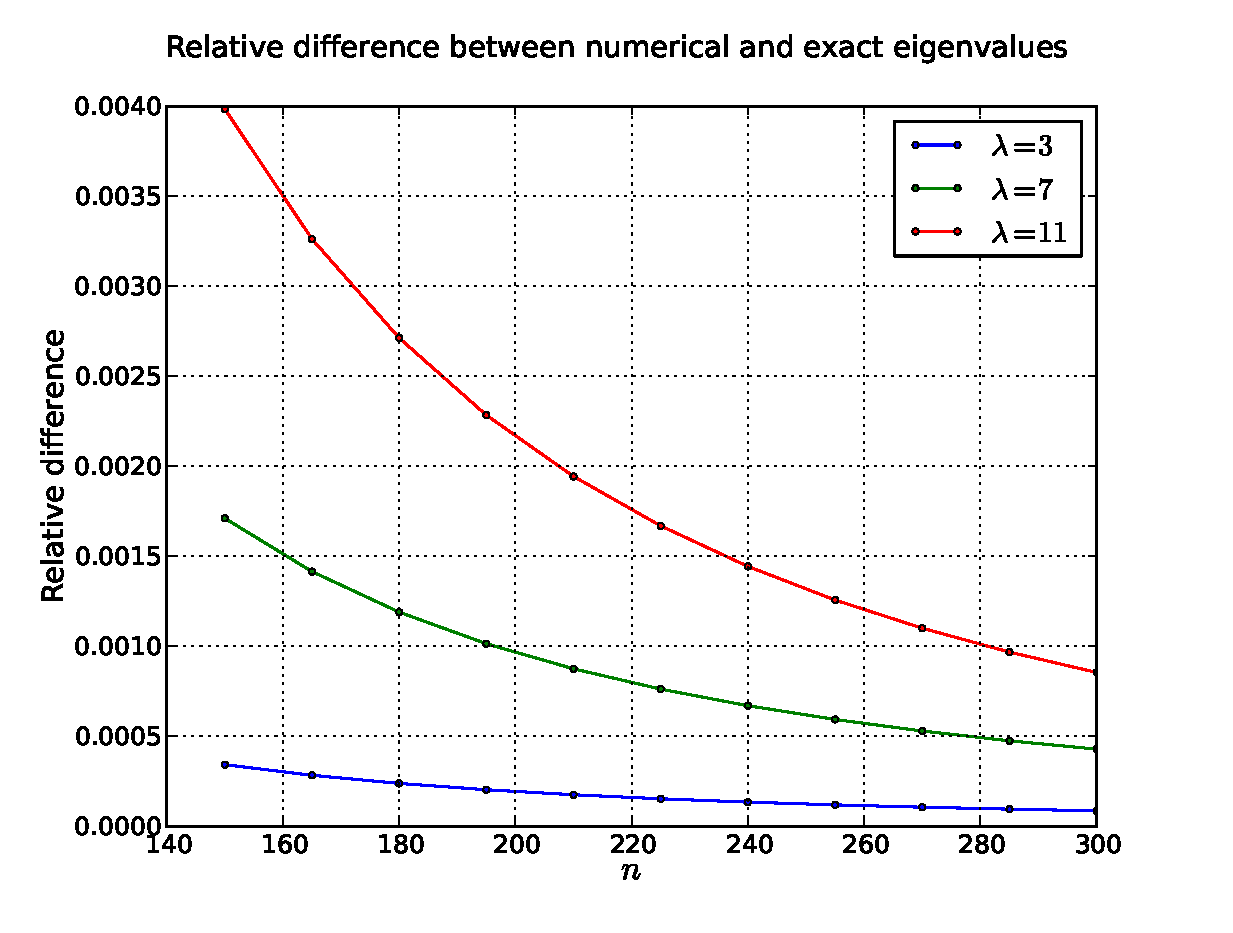
\includegraphics[width=1.0\textwidth]{images/nreldiff2.eps}
\caption{The figure shows how much the numerical eigenvalues differ from the analytical
	ones as $n_{step}$ increases.}
\label{fig:nreldiff}
\end{figure}
%





